% A LaTeX (non-official) template for ISAE projects reports
% Copyright (C) 2014 Damien Roque
% Version: 0.2
% Author: Damien Roque <damien.roque_AT_isae.fr>

\documentclass[a4paper,12pt]{book}
\usepackage[utf8]{inputenc}
\usepackage[T1]{fontenc}
\usepackage[english]{babel} % If you write in English
\usepackage{a4wide}
\usepackage{graphicx}
\graphicspath{{images/}}
\usepackage{subfig}
\usepackage{tikz}
\usetikzlibrary{shapes,arrows}
\usepackage{pgfplots}
\pgfplotsset{compat=newest}
\pgfplotsset{plot coordinates/math parser=false}
\newlength\figureheight
\newlength\figurewidth
\pgfkeys{/pgf/number format/.cd,
set decimal separator={,\!},
1000 sep={\,},
}
\usepackage{ifthen}
\usepackage{ifpdf}
\usepackage{enumitem}
\ifpdf
\usepackage[pdftex]{hyperref}
\else
\usepackage{hyperref}
\fi
\usepackage{color}
\usepackage{gensymb}
\hypersetup{%
colorlinks=true,
linkcolor=black,
citecolor=black,
urlcolor=black}

\renewcommand{\baselinestretch}{1.05}
\usepackage{fancyhdr}
\pagestyle{fancy}
\fancyfoot{}
\fancyhead[LE,RO]{\bfseries\thepage}
\fancyhead[RE]{\bfseries\nouppercase{\leftmark}}
\fancyhead[LO]{\bfseries\nouppercase{\rightmark}}
\setlength{\headheight}{15pt}
\usepackage{svg}
\let\headruleORIG\headrule
\renewcommand{\headrule}{\color{black} \headruleORIG}
\renewcommand{\headrulewidth}{1.0pt}
\usepackage{colortbl}
\arrayrulecolor{black}

\fancypagestyle{plain}{
  \fancyhead{}
  \fancyfoot[C]{\thepage}
  \renewcommand{\headrulewidth}{0pt}
}

\makeatletter
\def\@textbottom{\vskip \z@ \@plus 1pt}
\let\@texttop\relax
\makeatother

\makeatletter
\def\cleardoublepage{\clearpage\if@twoside \ifodd\c@page\else%
  \hbox{}%
  \thispagestyle{empty}%
  \newpage%
  \if@twocolumn\hbox{}\newpage\fi\fi\fi}
\makeatother

\usepackage{needspace}

\usepackage{amsthm}
\usepackage{amssymb,amsmath,bbm}
\usepackage{array}
\usepackage{bm}
\usepackage{multirow}
\usepackage[footnote]{acronym}
\usepackage{booktabs}

\newcommand*{\SET}[1]  {\ensuremath{\mathbf{#1}}}
\newcommand*{\VEC}[1]  {\ensuremath{\boldsymbol{#1}}}
\newcommand*{\FAM}[1]  {\ensuremath{\boldsymbol{#1}}}
\newcommand*{\MAT}[1]  {\ensuremath{\boldsymbol{#1}}}
\newcommand*{\OP}[1]  {\ensuremath{\mathrm{#1}}}
\newcommand*{\NORM}[1]  {\ensuremath{\left\|#1\right\|}}
\newcommand*{\DPR}[2]  {\ensuremath{\left \langle #1,#2 \right \rangle}}
\newcommand*{\calbf}[1]  {\ensuremath{\boldsymbol{\mathcal{#1}}}}
\newcommand*{\shift}[1]  {\ensuremath{\boldsymbol{#1}}}

\newcommand{\eqdef}{\stackrel{\mathrm{def}}{=}}
\newcommand{\argmax}{\operatornamewithlimits{argmax}}
\newcommand{\argmin}{\operatornamewithlimits{argmin}}
\newcommand{\ud}{\, \mathrm{d}}
\newcommand{\vect}{\text{Vect}}
\newcommand{\sinc}{\ensuremath{\mathrm{sinc}}}
\newcommand{\esp}{\ensuremath{\mathbb{E}}}
\newcommand{\hilbert}{\ensuremath{\mathcal{H}}}
\newcommand{\fourier}{\ensuremath{\mathcal{F}}}
\newcommand{\sgn}{\text{sgn}}
\newcommand{\intTT}{\int_{-T}^{T}}
\newcommand{\intT}{\int_{-\frac{T}{2}}^{\frac{T}{2}}}
\newcommand{\intinf}{\int_{-\infty}^{+\infty}}
\newcommand{\Sh}{\ensuremath{\boldsymbol{S}}}
\newcommand{\C}{\SET{C}}
\newcommand{\R}{\SET{R}}
\newcommand{\Z}{\SET{Z}}
\newcommand{\N}{\SET{N}}
\newcommand{\K}{\SET{K}}
\newcommand{\reel}{\mathcal{R}}
\newcommand{\imag}{\mathcal{I}}
\newcommand{\cmnr}{c_{m,n}^\reel}
\newcommand{\cmni}{c_{m,n}^\imag}
\newcommand{\cnr}{c_{n}^\reel}
\newcommand{\cni}{c_{n}^\imag}
\newcommand{\tproto}{g}
\newcommand{\rproto}{\check{g}}
\newcommand{\LR}{\mathcal{L}_2(\SET{R})}
\newcommand{\LZ}{\ell_2(\SET{Z})}
\newcommand{\LZI}[1]{\ell_2(\SET{#1})}
\newcommand{\LZZ}{\ell_2(\SET{Z}^2)}
\newcommand{\diag}{\operatorname{diag}}
\newcommand{\noise}{z}
\newcommand{\Noise}{Z}
\newcommand{\filtnoise}{\zeta}
\newcommand{\tp}{g}
\newcommand{\rp}{\check{g}}
\newcommand{\TP}{G}
\newcommand{\RP}{\check{G}}
\newcommand{\dmin}{d_{\mathrm{min}}}
\newcommand{\Dmin}{D_{\mathrm{min}}}
\newcommand{\Image}{\ensuremath{\text{Im}}}
\newcommand{\Span}{\ensuremath{\text{Span}}}

\newtheoremstyle{break}
  {11pt}{11pt}%
  {\itshape}{}%
  {\bfseries}{}%
  {\newline}{}%
\theoremstyle{break}

%\theoremstyle{definition}
\newtheorem{definition}{Définition}[chapter]

%\theoremstyle{definition}
\newtheorem{theoreme}{Théorème}[chapter]

%\theoremstyle{remark}
\newtheorem{remarque}{Remarque}[chapter]

%\theoremstyle{plain}
\newtheorem{propriete}{Propriété}[chapter]
\newtheorem{exemple}{Exemple}[chapter]

\parskip=5pt
%\sloppy

\begin{document}

%%%%%%%%%%%%%%%%%%
%%% First page %%%
%%%%%%%%%%%%%%%%%%

\begin{titlepage}
\begin{center}


\includegraphics[width=0.6\textwidth]{uol}\\[1cm]

{\large Deutsches Zentrum für Luft und Raumfahrt - Institut für vernetzte Energiesysteme}\\[0.5cm]

{\large Praxis-Seminar Modellierungsstudie}\\[0.5cm]

% Title
\rule{\linewidth}{0.5mm} \\[0.4cm]
{ \huge \bfseries Comparison of Two Optimization Methods for Operating a Smart Home Power Grid\\[0.4cm] }
\rule{\linewidth}{0.5mm} \\[1.5cm]

% Author and supervisor
\noindent
\begin{minipage}{0.4\textwidth}
  \begin{flushleft} \large
    \emph{Author}\\
    Tjark Smalla\\
  \end{flushleft}
\end{minipage}%
\begin{minipage}{0.4\textwidth}
  \begin{flushright} \large
    \emph{Professor} \\
    PD. Jan Freund
  \end{flushright}
\end{minipage}

\noindent
\begin{minipage}{0.8\textwidth}
	\begin{flushright} \large
		\vspace{\baselineskip}
		\emph{Supervisor} \\
		Dr. Peter Klement \\
		Dr. Patrick Schönfeldt \\
		Stefan Arens
	\end{flushright}
\end{minipage}

\vfill

% Bottom of the page
{\large \today}

\end{center}
\end{titlepage}

%%%%%%%%%%%%%%%%%%%%%%%%%%%%%
%%% Non-significant pages %%%
%%%%%%%%%%%%%%%%%%%%%%%%%%%%%

\frontmatter

\tableofcontents

\clearpage
\listoffigures

\clearpage
\chapter*{Acronyms}
\begin{acronym}[CP-OFDMX] % Give the longest acronym here
\acro{DER}{Distributed Energy Resource}
\acro{PV}{Photovoltaic}
\acro{MILP}{Mixed Integer Linear Programming}
\acro{OEMOF}{Open Energy Modelling Framework}
\acro{DLR}{Deutsches Institut für Luft und Raumfahrt}
\acro{SD}{Supply/Demand}
\acro{SDM}{Supply and Demand Matcher}
\acro{COP}{Coefficient of Performance}
\end{acronym}

%%%%%%%%%%%%%%%%%%%%%%%%%%%%%%%%%%%%%%%%%%%%
%%% Content of the report and references %%%
%%%%%%%%%%%%%%%%%%%%%%%%%%%%%%%%%%%%%%%%%%%%

\mainmatter
\pagestyle{fancy}

\cleardoublepage
\chapter{Introduction}\label{ch/intro}
 % Why is it important to optimize
 % Current Situation
According to a report of the European Comission 26,7\% of total energy consumption is caused by private households \cite{schedulingMilp}.
Due to the introduction of \ac{DER}s, private households are able to some of their demand by themselves.
However, power generation from renewables and household demand usually do not occur at the same time. To account for this, energy can be stored in e.g. batteries or used to fulfill demands in different sectors like the heating sector.
Scheduling power consumption and generation of connected devices (including batteries) in a home network is one of the requirements of the so called Demand Side Management.

Different methods to create these schedules already exist. One way to differ between them is by their scheduling horizon. 
The longer the scheduling horizon, the higher the uncertainties in the underlying predictions from e.g. the \ac{PV} forecast\cite{strategicScheduling}.

In the following report, two methods for creating such a schedule will be analyzed and their performance will be compared.
The first method is usually used for scheduling horizons greater than or equal to one day. In contrast to the first, the second method uses near real time scheduling. The simulations are performed by the \ac{OEMOF} and the HAL python frameworks.
Section \ref{s/intr/oemof} and \ref{s/intr/hal} introduce both methods in detail.
Chapter \ref{ch/methodology} explains in depth the tested home network (\ref{s/meth/grid}), the used time series (\ref{s/meth/ts}), the performance metrics (\ref{s/meth/pfm}) and the analyzed test setups (\ref{s/meth/setup}).
In the last two chapters \ref{ch/results} and \ref{ch/conclusion}, results are analyzed and conclusions about the properties of each method are made.


\section{OEMOF in Detail}\label{s/intr/oemof}
In the first method, an energy system is modeled as an \ac{MILP} problem. This is then solved by one of the most efficient general purpose \ac{MILP} solvers today, the branch-and-cut algorithm\cite{branchAndCutEfficient}. An optimal energy system control schedule for the given initial conditions can be extracted from the result of the optimization.

Although iterative applications of this method exist, it is usually used for scheduling horizons greater or equal to one day\cite{strategicScheduling}\cite{schedulingMilp}.

The \ac{OEMOF} framework provides the user with a set of components to model an energy system. Section \ref{s/meth/comparability} describes in more detail which subset of those components are used in the comparison. The online documentation provides a complete list of all available components. \cite{oemofDoc}
The power flow is simulated along the edges of a bipartite graph which contains the before mentioned components as nodes.

Although the whole set of rules to generate the \ac{MILP} problem from the component graph can not be covered by this report, the reader should get an intuition reading section \ref{s/intr/oemof/milp}. For further research, the official paper is recommended. \cite{oemof}

\subsection{Generating a MILP Problem from OEMOF Components}\label{s/intr/oemof/milp}
A \ac{MILP} problem is made up of a set of linear inequalities and linear equalities $A$, and an objective function $c^Tx$. The problem aims to find the solution vector $x$ which minimizes the objective function while fulfilling  $Ax \leq b$,  $x \geq 0$ and $x_j \in \mathbb{Z}, \forall j \in J$. As a consequence of the last term, the solution vector $x$ can be, but is not limited, to integers.

In the modeled energy system $x$ holds the state of the system (e.g. power flow between two nodes or a battery charge) at a certain point in time $t$. The physical constraints are represented by $A$ and $b$. An example for such a constraint would be the maximal power flow allowed between two components\footnote{Limited for example by the cable diameter}. Besides user generated constraints, \ac{OEMOF} introduces some static constraints inherent to an energy system. An example would be the requirement to have net power flow of 0 in the whole system (no energy flows out or into the system).

The objective function seen in equation \ref{e/intr/objectiveFunction1} is made up of costs $c$ which are generated by the (sometimes time dependent) states of the edges and nodes of the graph. An example node in the graph could be a power plant which generates costs according to the amount of power fed into the network at a certain time step of the simulation. Such an optimization state of a component is in the following referred to as degree of freedom of the component.
Equation \ref{e/intr/objectiveFunctionNodeTime} provides an intuition how the simulation time has a significant impact on matrix and vector size of the problem and thus, on hardware requirements for the simulation.
The cost function is given by
\begin{equation}\label{e/intr/objectiveFunction1}
	min: \sum_{t\in T}e(t)+\sum_{t\in T}^{}n(t) 
	+ \sum_{(s,e)\in E}\sum_{i\in I_2}c^i_{(s,e)}\cdot w^i_{(s,e)}
	+ \sum_{n\in N}\sum_{i\in I_4}c^i_{n}\cdot v^i_{n}
\end{equation}
\begin{equation}\label{e/intr/objectiveFunctionNodeTime}
n(t)=\sum_{n\in N}\sum_{i\in I_1}c^i_n(t)\cdot v^i_n(t)\cdot \tau
\end{equation}
\begin{equation}\label{e/intr/objectiveFunctionEdgeTime}
e(t)=\sum_{(s,e)\in E}\sum_{i\in I_1}c^i_{(s,e)}(t)\cdot w^i_{(s,e)}(t)\cdot \tau
\end{equation}

where $w$ and $v$ are the state of edges and nodes, $N$ and $E$ are the sets of nodes and edged, $I_i$ are different cost sets, $T$ is the simulation time and $\tau$ the time between to time steps.

\section{HAL in Detail}\label{s/intr/hal}
The algorithm called HAL was developed at the \ac{DLR} Institute of Networked Energy Systems by Stefan Arens.
It implements a market based control concept for supply and demand matching utilizing a continuous japanese auction. 
A similar concept was already proven to smoothen the net import profile of an energy system and is thus a promising method for controlling decentralized energy systems with high share of distributed generation\cite{powermatcher}. Although, theoretically the auction can be performed in arbitrary intervals, it was designed and tested for short scheduling horizons. For this report, an interval of one minute is chosen.

HAL users model their energy system by building a tree structure out of components. HAL distinguishes between two types of nodes: \ac{SDM} and devices.
A \ac{SDM} node performs a japanese auction on its child nodes. A device node implements a \ac{SD} function modeled after the physical features of the device it is supposed to represent. Section \ref{s/intr/hal/auction} explains the auction algorithm in more detail.
The only requirement imposed on the implemented \ac{SD} functions is monotonicity. This ensures that the \ac{SDM} can control the market to either generate or consume more power, depending on the overall market situation.
The children of an \ac{SDM} can be devices but also other \ac{SDM}. \ac{SDM} at the bottom of the tree resolve sub markets first before communicating the resulting sub market demand to their parent \ac{SDM}. 
Section \ref{s/intr/hal/auction} explains in more detail how the matchers try to achieve a target in their sub market.
If each matcher achieves its goal, the energy system is in a favorable state in which the necessary net power import is zero. \cite{schedulingMilp}

\subsection{Auction Algorithm}\label{s/intr/hal/auction}
In each time step, each \ac{SDM} in the tree performs an auction in their sub market.
The sub market is controlled by a virtual price signal $p \in [0, 100]$ on which the matchers children $c$ react with a proposal of how much power $q \in \mathbb{R}$ they consume or generate according to their supply and demand function $q_c(p)$. A negative quantity indicates generation rather than consumption. 

At the start of each auction in each time step $t$, the matcher sends a neutral price signal of $p_0=50$ to all of its children. They react with the quantity of power they would consume or generate for this price. 
The matcher then alters its price signal for the next iteration to get closer to its target of $q=0$. 
Because of the monotonicity of all involved \ac{SD} functions, it is safe to assume that consumption will increase when the price is lowered.
For clarification, equation \ref{e/int/hal/min} displays the building rule applied in each iteration to create the next price signal where $q_i$ is the sum of all supply/demand proposals received from the matchers children nodes $c$.

\begin{equation}\label{e/int/hal/min}
\begin{split}
q_i = \sum_{c \in C} q_c(p_i)\\
p^t_{i+1}  = p_i + s^t_i \\
s^t_i = \begin{cases}
1 ,& \text{if } q_i \geq 0\\
-1,& \text{else}
\end{cases} \\
\end{split}
\end{equation}

The auction is closed as soon as 
\begin{equation}\label{e/hal/closingCondition}
	q_i = 0 \lor |q_i| > |q_{i-1}| \lor p \in \{0, 100\}
\end{equation}
holds. When the auction is closed and $q_i \neq 0$, the last iteration increased the distance to the target and thus $p_{i-1}$ is considered the optimal price for this timestep.

% --------------------------------------------------------------------------------------------
\chapter{Methodology}\label{ch/methodology}
This chapter provides an overview about the test setup used to compare both algorithms explained in section \ref{s/intr/oemof} and \ref{s/intr/hal}.
For both algorithms, an energy system has to be modeled. In order to compare them, these systems have to be as similar as possible.
Section \ref{s/meth/comparability} discusses how both systems are modeled to ensure comparability despite the different approaches of the algorithms used.
Based on these actions, section \ref{s/meth/grid} gives an overview about the simulated energy system which uses time series briefly explained in section \ref{s/meth/ts}.
The performance metrics used for the comparison are explained in section \ref{s/meth/pfm}.
Finally, section \ref{s/meth/setup} explains the different test setups tested.

\section{Ensuring Model Comparability}\label{s/meth/comparability}
To ensure comparability of both systems, the components used in both frameworks were required to have a counterpart in the other framework.
The only detail in which they are allowed to differ is the usage of the degree of freedom introduced in section \ref{s/intr/oemof/milp}.
A list with all used components and their implementations in both frameworks is given in \ref{s/meth/comp/components}.
To ensure that both simulations run with the same parameters at all time, the system under test is modeled in \ac{OEMOF} and then converted into a HAL model with the same parameters.
For implementation details please refer to the $hal\_plugin$ folder in the appended python code base.

The \ac{OEMOF} framework optimizes costs whereas HAL optimizes on a net import/export of zero.  
In order to force \ac{OEMOF} to optimize the net import as well, imported and exported power from the modeled system creates costs. Both components are further described in section \ref{s/meth/grid}.

\subsection{Used components}\label{s/meth/comp/components}
This sections lists all used abstract components and their respective implementations in both frameworks.

\subsubsection{Consumer and Generators}
Consumer and Generators are components which either draw or feed power.
Although in theory they could, in the context of this report they have no degree of freedom for the simulation.
They are used to provide time dependent power consumption/generation.

\begin{itemize}
	\item Name in \ac{OEMOF}: Sink, Source
	\item Name in HAL: InelasticBehavior
	\item Parameter: Power consumption/generation(t)
	\item Degrees of Freedom: -
\end{itemize}


\subsubsection{Storage}
In one time step storages can consume energy which they later provide in another time step. 
In the test system, they are used as simple models for batteries as well as for thermal energy storages.
However, a storage can only store energy up to its capacity $c^{max}$.
The amount of energy stored in a storage is denoted by $c$.
it is governed by
\begin{equation}
	c_t = min(c^{max}, c_{t-1} + \eta \tau (P_t^{in} - P_t^{out})) 
\end{equation} with the conversion factor $\eta$, the simulation interval $\tau$ and the power flow $p$.
The amount of energy the storage can produce/consume in one time step is limited by $p^{max}$.

\begin{itemize}
	\item Name in \ac{OEMOF}: Generic Storage
	\item Name in HAL: Battery
	\item Parameters: $\eta$, $c^{max}$, $P^{max}$
	\item Degrees of Freedom: $P_t^{in}, P_t^{out}$
\end{itemize}

\subsubsection{Transformer}
A transformer is able to connect two energy sectors.
It is used as a highly simplified model for sector coupling between power sector and thermal sector. Such a coupling is often achieved by a heat pump. A heat pump usually produces more thermal energy and it consumed of electric energy. This relation is given by its \ac{COP}. To further model the properties of a heat pump, energy flow is only allowed from electrical to thermal energy.

In HAL this is implemented by a \ac{SDM} which optimizes the amount of power generated by itself instead of a net import/export of zero.

The transformed energy is calculated by $E^{transformed}_t = P^{in}_{t} \cdot COP \cdot \tau$.

\begin{itemize}
	\item Name in \ac{OEMOF}: Transformer
	\item Name in HAL: Parent Transformer
	\item Parameters: $COP$
	\item Degrees of Freedom: $P^{in}_{t}$
\end{itemize}

\section{Tested Energy System}\label{s/meth/grid}
The tested energy system is supposed to represent an average household in the north of Germany.
Power is generated by a \ac{PV} system and consumed by common activities of the residents referred to as the household load.
The power system is connected to a local thermal energy system by a heat pump. 
The thermal energy system itself also consists of a thermal storage and a thermal load.

\section{Time Series}\label{s/meth/ts}
% >>> pred = pd.read_csv('../hal_plugin/data/2016_pred_res60s_7days_train_full.csv', parse_dates=True, index_col=0)
% >>> real = pd.read_csv('../hal_plugin/data/2016_real_res60s_7days_train_full.csv', parse_dates=True, index_col=0)
% >>> pv = pd.read_csv('../hal_plugin/data/ol_data_pv_az180_inc36_mod23.csv', parse_dates=True, index_col=0)
% >>> heat = pd.read_csv('../hal_plugin/data/sh_intensity=15_area=46.5.csv', parse_dates=True, index_col=0)
% >>> load = pd.read_csv('../hal_plugin/data/SumProfiles.Electricity_processed.csv', parse_dates=True, index_col=0)
% [ax.set_ylabel('W') for ax in pd.DataFrame({'2016_pred_res60s_7days_train_full.csv': pred['power[W]'], "2016_real_res60s_7days_train_full.csv": real['power[W]'], "ol_data_pv_az180_inc36_mod23.csv": pv['power[W]'], "sh_intensity=15_area=46.5.csv": heat['E [kWh]'] * 1000 / (1 / 60), "SumProfiles.Electricity_processed.csv": load['power[W]']}, index=load.index).plot(subplots=True, sharey=True, title='Time Series Overview')]
% For time series overview from cwd = hal
The time series used for the simulation are either provided by the \ac{DLR} or generated by the Load Profile Generator\footnote{https://www.loadprofilegenerator.de/}. The Load Profile Generator simulates peoples activities triggered by their daily needs. Each activity can consume power or thermal energy as warm water. It was used to create the power load profile for the simulated household.
The following is a comprehensive list of each used data source in the simulation: 

\begin{itemize}
	\item 2016\_pred\_res60s\_7days\_train\_full.csv - Predicted output of a \ac{PV} system in Oldenburg generated by the algorithm described in \cite{dlrPred}
	\item 2016\_real\_res60s\_7days\_train\_full.csv - Actual \ac{PV} output for the in 2016\_pred\_res60s\_7days\_train\_full.csv predicted system
	\item ol\_data\_pv\_az180\_inc36\_mod23.csv - Actual \ac{PV} output of an Oldenburg located \ac{PV} system.
	\item sh\_intensity=15\_area=46.5.csv - Thermal load based on degree days. Section \ref{s/meth/thermal} describes this in more detail.
	\item SumProfiles.Electricity\_processed.csv - Power load generated by the Load Profile Generator
\end{itemize}
Each time series can be found in the appended codebase in the folder $hal\_plugin/data$.

In order to additionally analyze the influence of sector coupling on algorithm performance, both algorithms are tested in two different time periods.
The simulation duration was set for both periods to one month. Figure \ref{f/meth/ts/overview} shows that available data limits the possible simulation periods to September 2016 to February 2017.
In order to analyze the impact of sector coupling on the result, two periods were chosen. One containing no thermal load and high \ac{PV} output and the other containing high thermal load and low \ac{PV} output.

\begin{figure}[htp]
	\centering
	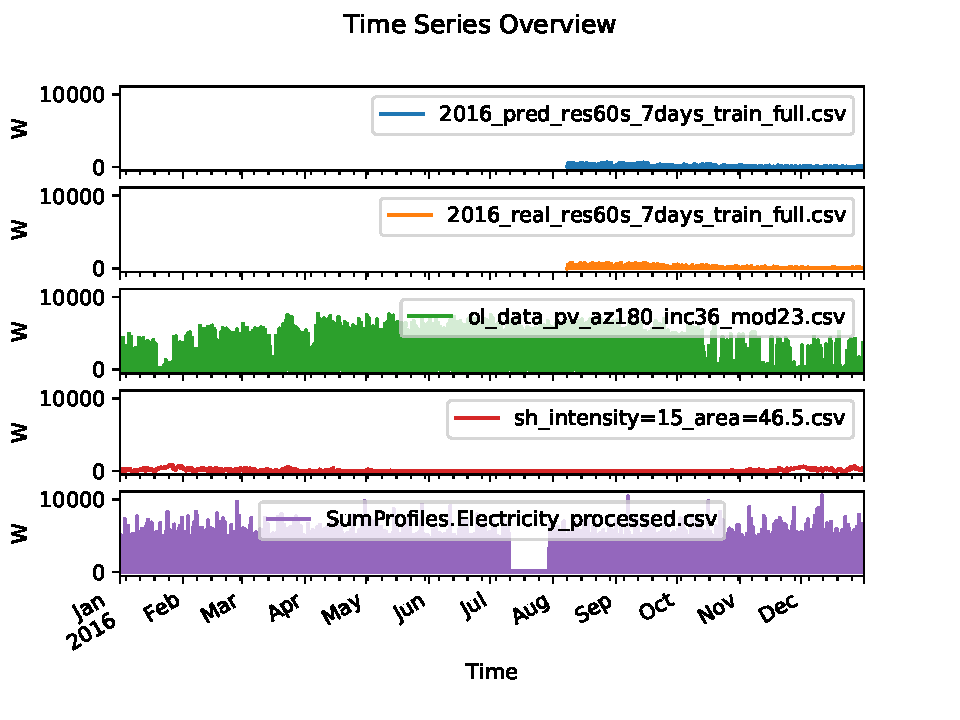
\includegraphics[width=\textwidth]{overview}
	\caption{Overview of used time series with energy consumption/generation in Watts. Due to missing data, feasible simulation periods are only September to December. September allows for simulations without sector coupling effects, because the thermal load is constantly zero.}
	\label{f/meth/ts/overview}
\end{figure}

\subsection{Thermal Load Model}\label{s/meth/thermal}
The thermal load was calculated using the degree day method.
A degree day $dd$ is  calculated by
\begin{equation}
	max(0, T_b - T_t) * \tau = dd
\end{equation}
where $T_r$ is the base temperature of the considered building, $T_t$ is the outside air temperature at time $t$ and $\tau$ is the time interval in days.

The power consumption per degree day $p^{dd}$ is then calculated by 
\begin{equation}
	p^{dd} = p^{year} / \sum_{t\in Y} dd_t
\end{equation}
with $Y$ being all degree day datapoints and $p^{year}$ being the total power consumed for heating during the period of the year .

\section{Relevant Performance Metrics}\label{s/meth/pfm}
As explained in chapter \ref{ch/intro}, a good schedule reduces the net power import and peak loads. 
A net power import is related to costs for the household. Further, all power imported from the grid leads to pressure on the infrastructure. A high net import should thus be avoided.
Because of this, the main performance metric is the net power import over the whole simulation time. Besides the total power import, abundance and intensity are indicators for the pressure put onto the grids infrastructure while controlling the system according to the generated schedules.

\section{Simulation Setup}\label{s/meth/setup}
To allow algorithm comparability, a python plugin which converts an \ac{OEMOF} energy system into a HAL configuration was developed.
Starting with a simple power network consisting only of consumers/generators and a storage, the plugin was further extended to allow for more complex simulations like the simulated sector coupling.

To create a baseline for the following simulations, a simple simulation is done using the energy system described in \ref{s/meth/grid} and the data described in \ref{s/meth/ts}. 

The file ol\_data\_pv\_az180\_inc36\_mod23.csv is used as input for the \ac{PV} system if not mentioned otherwise.
Both algorithms performances are compared according to the metrics defined in section \ref{s/meth/pfm}.

One of the main research question is the dependence of \ac{OEMOF} generated schedules on its scheduling horizon.
By slicing \ac{OEMOF}s optimization problem into multiple smaller problems, the schedule horizon can be shortened.
In the following, this setup is referred to as incremental setup.

To analyze both algorithms dependence on the correctness of the models input data, three additional setups are simulated.
In each setup, the baseline simulation is performed with both algorithms using a certain set of parameters.
Section \ref{s/meth/schedule} explains how an energy system control schedule is generated from this first baseline simulation.
This schedule is then used to control the \ac{OEMOF} energy system in a second simulation.
Except for the \ac{PV} systems output data and the schedule controlled component behavior, the second simulation equals the first.
Because of HALs short schedule horizon of one minute, it is not used to create a control schedule, but as an online system controller in the first and the second simulation.

% Noise setup
For the second simulation setup, noise is induced into the \ac{PV} data of the second simulation step. The noises standard deviation is then increased to analyze a potential correlation between schedule performance and input disparity during schedule creation and application. In the following this simulation setup is referred to as noise setup. For each standard deviation, an ensemble of 10 simulation runs is performed to mitigate random effects.

% Real Data Setup
In the third setup, the baseline simulation from which the schedule is created, is based on \ac{PV} prediction data. The schedule is then used to control a system which is fed by the actual \ac{PV} data for the same time period the prediction was made for. HAL is used both times as an online controller. In the following, this setup is referred to as real data setup.

% Schedule vs Schedule 
The fourth setup equals the third, but HAL is not used as an online controller. Instead, the system in the second simulation step is controlled by a schedule. This way both algorithm's ability to create a performant schedule for offline system controlling is analyzed. In the following this setup is referred to as schedule vs. schedule setup.

\section{Creating a Schedule from Simulation Output}\label{s/meth/schedule}
Output of both algorithms is the power consumption/generation of each device at each time step of the simulation.
In a second simulation step the devices can be controlled by this information to mimic their behavior from the previous run.

The second simulation step is also performed by using the \ac{OEMOF} framework.
Offline system control is achieved by replacing the degrees of freedom of the simulation graph by the fixed behavior from the previous simulation run.
A storage for example is replaced by a source node and a sink node which are configured to feed or draw power according to the storage behavior of the first simulation run.

\subsection{Noise Induced PV Data}
Equation \ref{e/meth/setup/noise} shows how the noise induced \ac{PV} power output $p^{noise}_i(t)$ consists of the sum of the time dependent \ac{PV} data from $ol\_data\_pv\_az180\_inc36\_mod23.csv$ $p(t)$ and the noise, generated by an Ohrnstein Uhlenbeck process $ou$ with a mean of zero, a fixed relaxation parameter $\tau$ and a given standard deviation $\sigma_i$. The output power is clipped at zero and the maximal possible power output of the \ac{PV} system $p^{max}$.

\begin{equation}\label{e/meth/setup/noise}
	p^{noise}_i(t) = min(p^{max}, max(0, p(t) + ou(t, 0, \sigma_i, \tau)))
\end{equation}

In comparison with \ac{OEMOF}s long term schedule, HALs performance is expected to increase with increasing difference between \ac{PV} data for schedule creation $p(t)$ and \ac{PV} data during system controlling $p^{noise}_i(t)$.

% --------------------------------------------------------------------------------------------
\chapter{Results}\label{ch/results}
All results discussed in this chapter are based on the simulation output which can be found in the appended codebase in the folder $result\_data$.
\newpage
\section{Baseline Results}
The results of the baseline setup discussed in \ref{s/meth/setup} are displayed in \ref{f/res/baseline/total} a$)$. As expected, \ac{OEMOF}s overall net import is with only 69\% of HALs total net import much lower. Although, the maximum net import peak of $0.174018$kW caused by HAL and $0.173485$kW caused by \ac{OEMOF} is similar, analyzing figure \ref{f/res/baseline/total} $b)$ reveals that peaks in  \ac{OEMOF}s simulation results are not as frequent as in HALs results.

\begin{figure}[htp]
 \centering
\subfloat[Above: Cummulated Net Import in kWh. Below: Total Net Import in kWh.]{{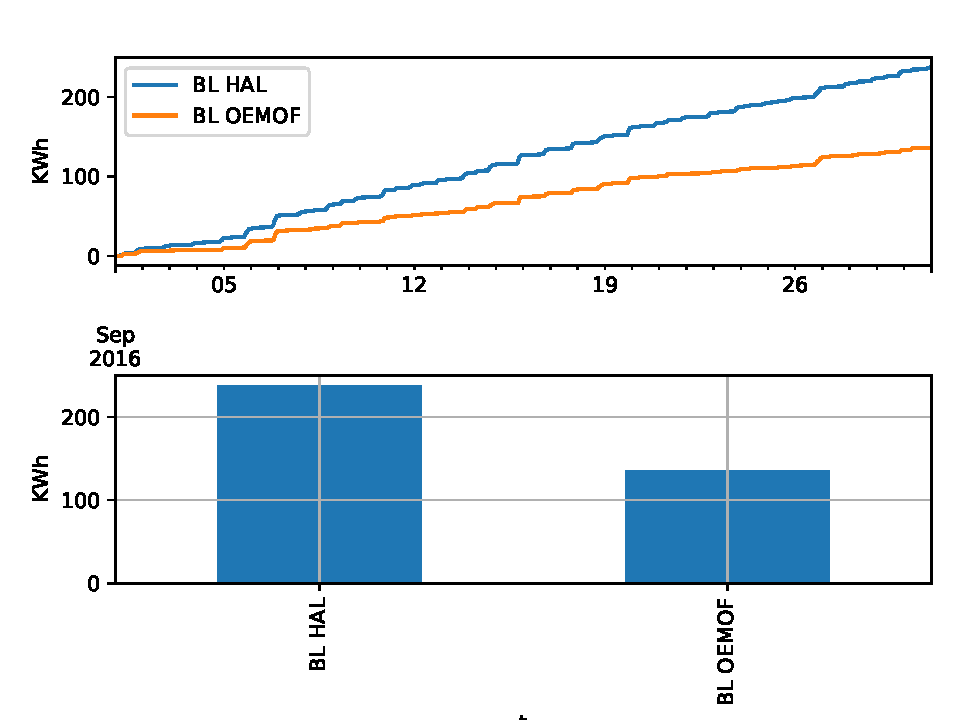
\includegraphics[width=0.465\textwidth]{baseline_pvol_total} }}%
\qquad
\subfloat[Net Import Peak Distribution. Whiskers are 1.5 of the inter quantile range.]{{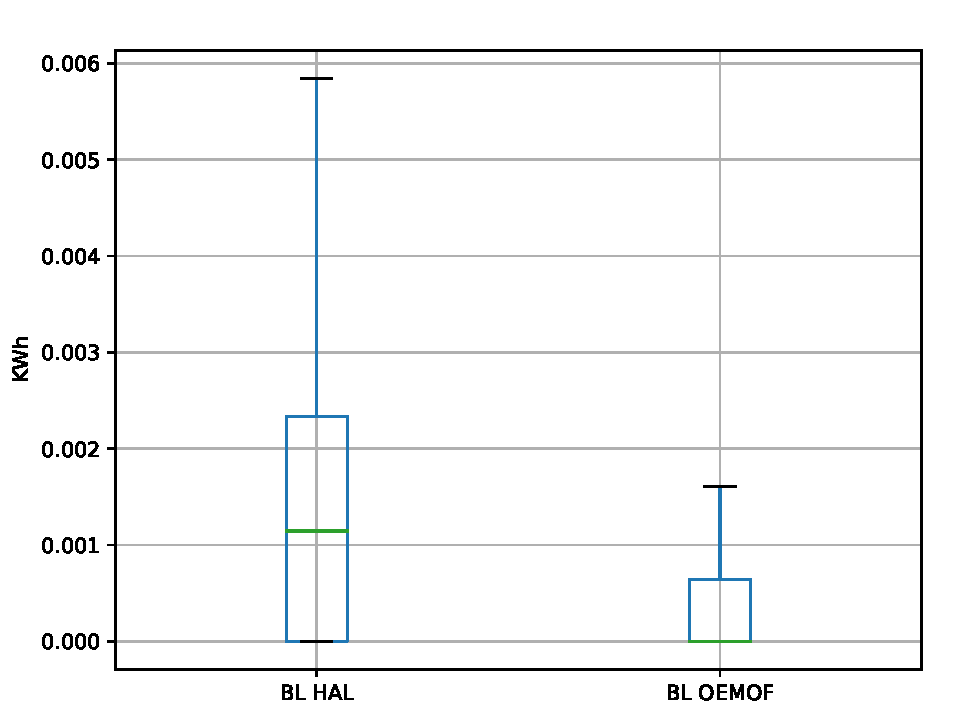
\includegraphics[width=0.465\textwidth]{baseline_pvol_peaks} }}%
\caption{The \ac{MILP} optimization with the \ac{OEMOF} framework caused less power import. If power is imported, the amount of power is usually small compared to HALs power imports.}%
\label{f/res/baseline/total}%
\end{figure}


\newpage
\section{Incremental Setup}
In the first simulation step a baseline simulation for the simulation period of September was performed.
In a second, third and fourth step, \ac{OEMOF}s scheduling horizon was reduced to 24, 12 and 6 hours. In the following, the net power import of all runs was compared.

Figure \ref{f/res/incr/total} shows that splitting the optimization problems increases the imported power amount and the occurrence of net power peaks. However, even the 6 hour \ac{OEMOF} optimization split performs better than controlling the energy system with the HAL algorithm.
	
The 1 day split with a net import of $136.26$kWh performs almost identical as the simulation without split and a net import of $135.44$kWh. Analyzing the behavior of the optimization problem in detail, this is likely because the only degree of freedom in these setup is the battery. 
In the evening, the household load increases and the \ac{PV} system generates no power. As a result the battery is used as energy producer during the evening until depleted. Thus each day the system starts with an empty battery.

\begin{figure}[ht]
	\centering
	\subfloat[Above: Cummulated Net Import in kWh. Below: Total Net Import in kWh.]{{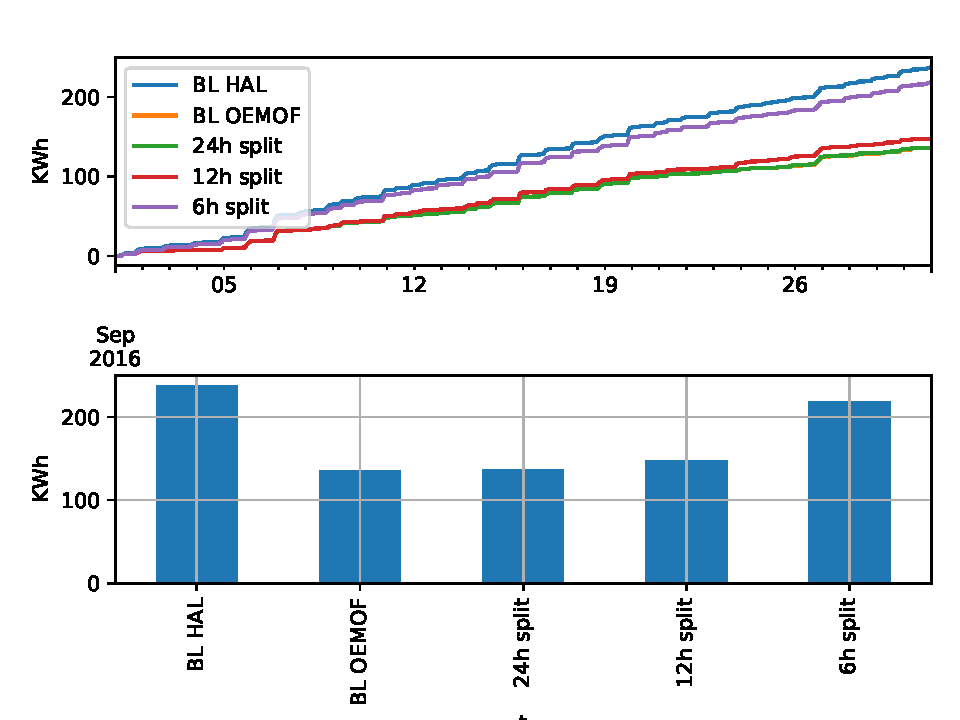
\includegraphics[width=0.465\textwidth]{splits_total} }} % %\includesvg{image}
%	\qquad
	\subfloat[Net Import Peak Distribution. Whiskers are 1.5 of the inter quantile range.]{{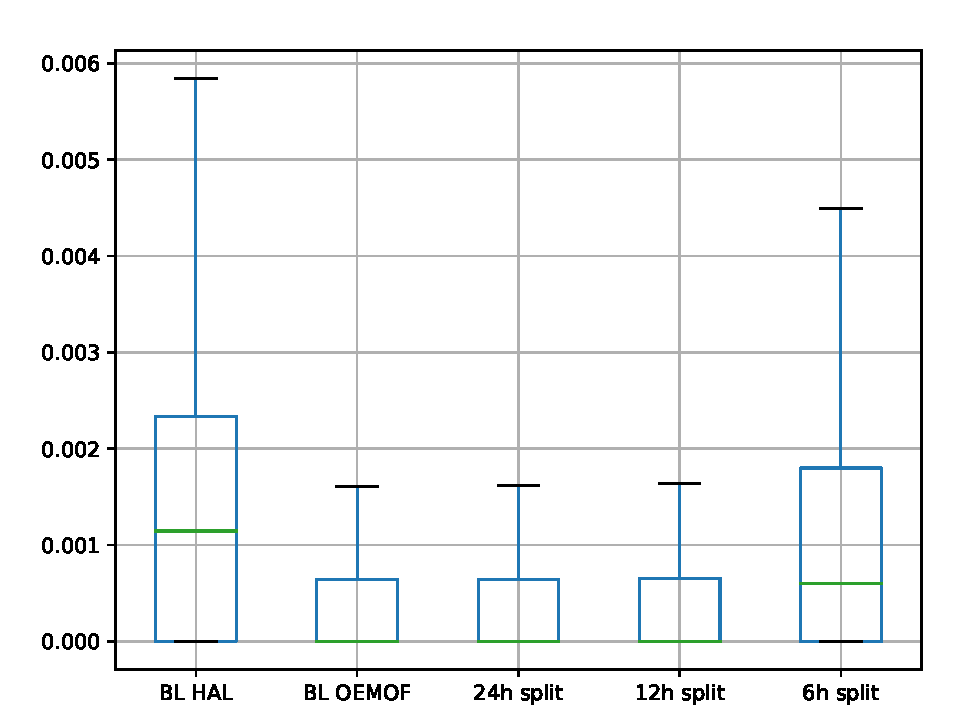
\includegraphics[width=0.465\textwidth]{splits_peaks} }}%
	\caption{Performance of \ac{OEMOF} optimized simulations decreases with short scheduling horizons. The biggest performance difference is between the 12h and 6h split. However, the 6h split performs better than the baseline simulation with the HAL algorithm.}%
	\label{f/res/incr/total}%
\end{figure}

\newpage
\section{Noise Setup}\label{s/res/noise}
In order to analyze the dependence of a schedule controlled energy system on the correctness of the input data used for schedule creation, the performance of a schedule on differently strong noised \ac{PV} input data was tested. Figure \ref{f/res/noise/total} shows how the net import of the schedule controlled systems increases with increasing noise variance. The stronger the deviation between input data used for schedule creation and input data during system control the bigger the necessary net import. 

\begin{figure}[htp]
	\centering
	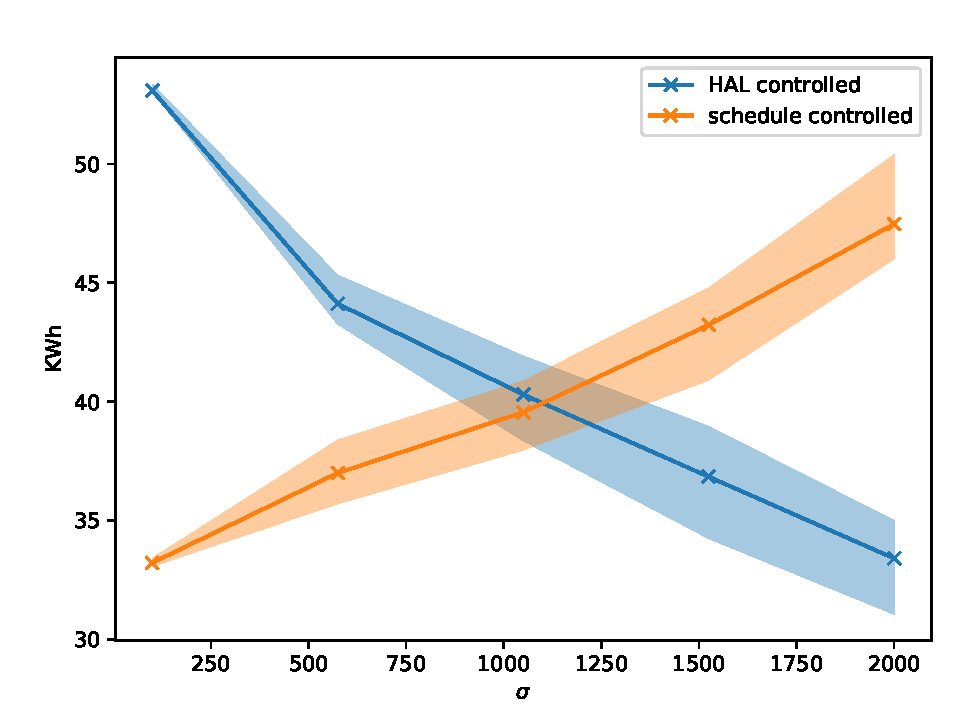
\includegraphics[width=\textwidth]{noiseTotalNet}
	\caption{Total net import for different noise standart deviations $\sigma$. The areas mark the 25 and 75 percentile of the ensemble runs. The solid lines mark the median of the ensemble runs. HALs import seems to be negatively correlated to $\sigma$ while OEMOFs import rises with increasing $sigma$.}
	\label{f/res/noise/total}
\end{figure}

Another interesting observation is the negative correlation between noise variance and the net import of the energy system controlled by HAL. This is likely caused by the additive noise. The resulting \ac{PV} output consists of the sum of the generated noise and real \ac{PV} data. As a result the \ac{PV} system produces power even during the night when in reality no sun would shine. The almost real time control behavior of HAL allows to use this additional power while the schedule controlled system does not expect and consume power in these times. Figure \ref{f/res/noise/noiseExample} shows how the PV output in the morning and evening is used by the HAL algorithm to load the storage.

\begin{figure}[htp]
	\centering
	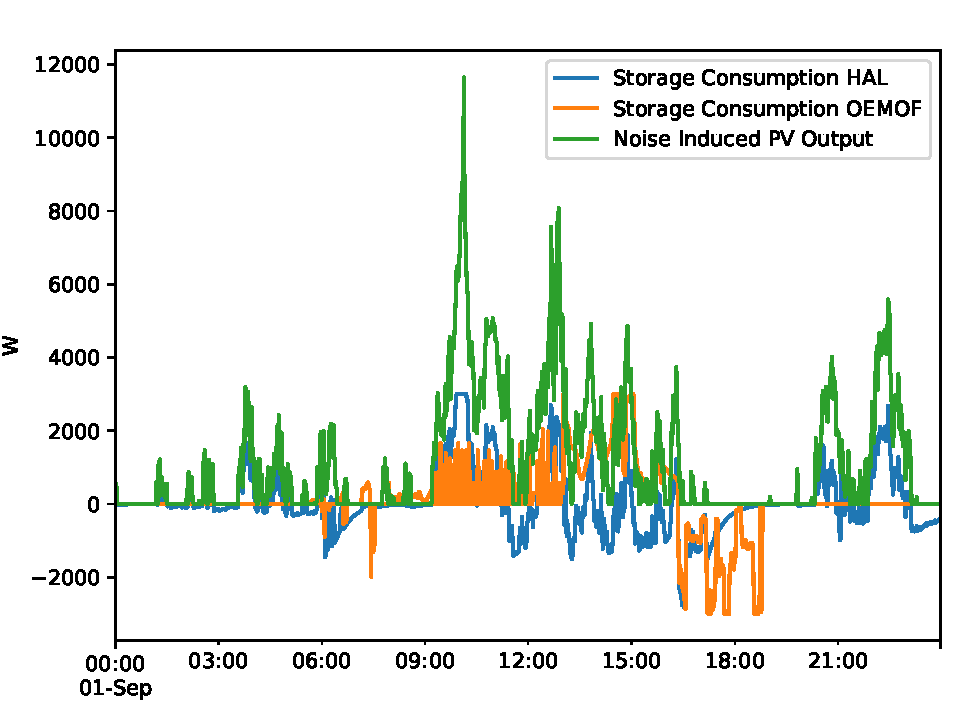
\includegraphics[width=\textwidth]{noiseExample}
	\caption{Power Flow during the first day of one ensemble run with $\tau = 30$ and $\sigma=2000$. }
	\label{f/res/noise/noiseExample}
\end{figure}
\newpage
\section{Real Data Setup}
The Noise Setup analyzed in \ref{s/res/noise} suggested that the HAL algorithm can adapt better to uncertainties in the input \ac{PV} data and thus achieve better performance than a schedule controlled approach. However, the model used for creating these uncertainties was far from a realistic situation. 
For a more realistic approach, a data pair of actual \ac{PV} data and its prediction was used in the real data setup. 
Although not as strong as in the noise setup, the same effects can be seen. Figure \ref{f/res/real/total} shows that the HAL algorithm improves its performance against the schedule controlled simulation during the September period. In the HAL controlled approach, the simulation performed with real \ac{PV} data achieved $2.16$\% less net power import. In contrast, the schedule controlled approach requires $0.76$\% more net import. The peak analysis shows also a slight improvement in the real data run with the HAL algorithm and a slight decline with the \ac{OEMOF} created schedule.
\begin{figure}[htp]
	\centering
	\subfloat[Total Net Import.]{{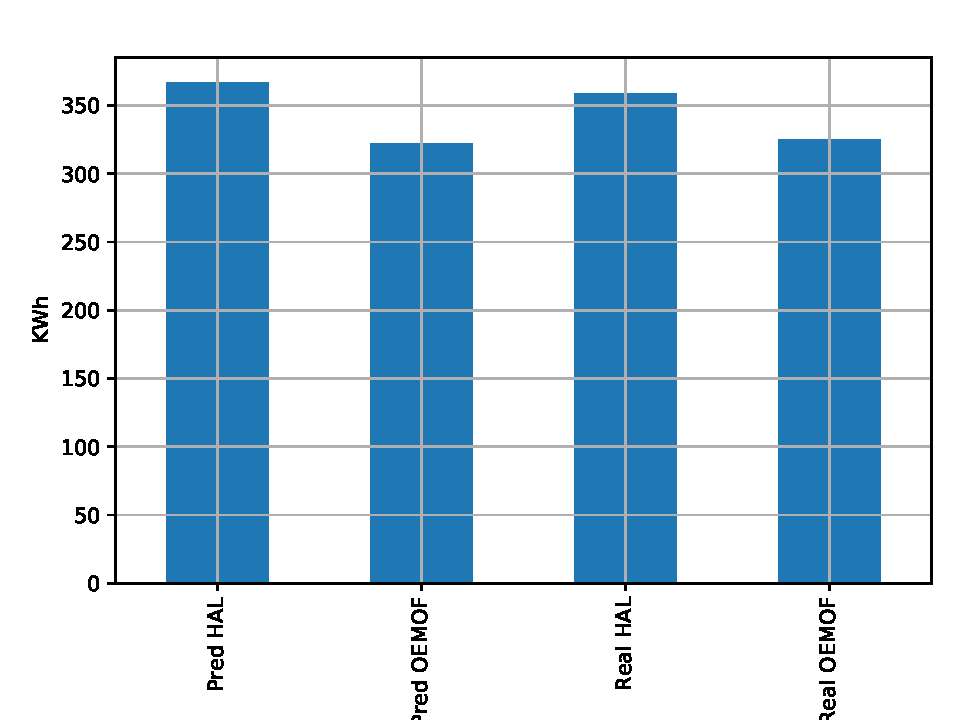
\includegraphics[width=0.465\textwidth]{sept_real_total} }} % %\includesvg{image}
	%	\qquad
	\subfloat[Net Import Peak Distribution. Whiskers are 1.5 of the inter quantile range.]{{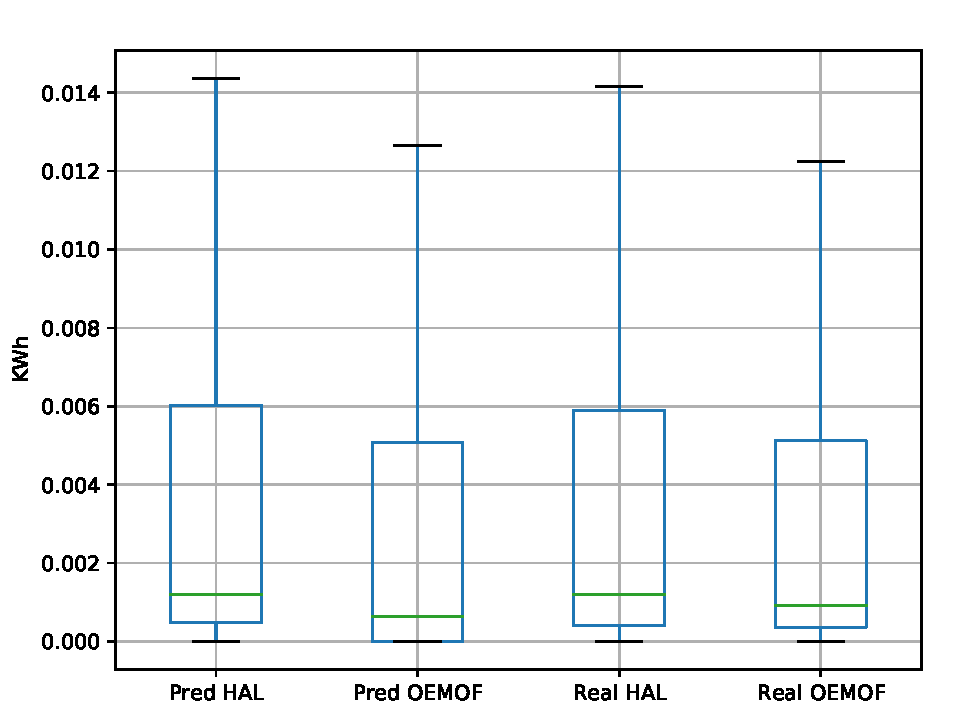
\includegraphics[width=0.465\textwidth]{sept_real_peaks} }}%
	\caption{Simulation results with real PV and prediction data for September. \ac{OEMOF}s first simulation run performs slightly better than the second which is controlled by a schedule. HAL is improving in the second run. HAL is used in both runs as a near realtime controller.}%
	\label{f/res/real/total}%
\end{figure}

As in the noise setup, the HAL algorithm can react to unforeseen changes and load the battery when \ac{PV} output is unexpectedly high. Besides the optical indication in figure \ref{f/res/real/example}, the correlation between \ac{PV} output and battery power consumption and generation is listed in table \ref{t/res/real}. The HAL controlled storage consumption correlates more with the actual \ac{PV} data than with the predicted one. In the schedule controlled simulation the situation is flipped.

\begin{table}
\centering
\caption{Correlation between PV input and storage consumption}
\label{t/res/real}
\begin{tabular}{lrrrr}
\toprule
{} &  HAL & Schedule & Pred PV & Actual PV \\
\midrule
HAL controlled Storage Balance      & 1.00 &     0.38 &    0.21 &      0.38 \\
Schedule controlled Storage Balance & 0.38 &     1.00 &    0.34 &      0.29 \\
Pred PV Output                      & 0.21 &     0.34 &    1.00 &      0.80 \\
Actual PV Output                    & 0.38 &     0.29 &    0.80 &      1.00 \\
\bottomrule
\end{tabular}
\end{table}


\begin{figure}[htp]
	\centering
	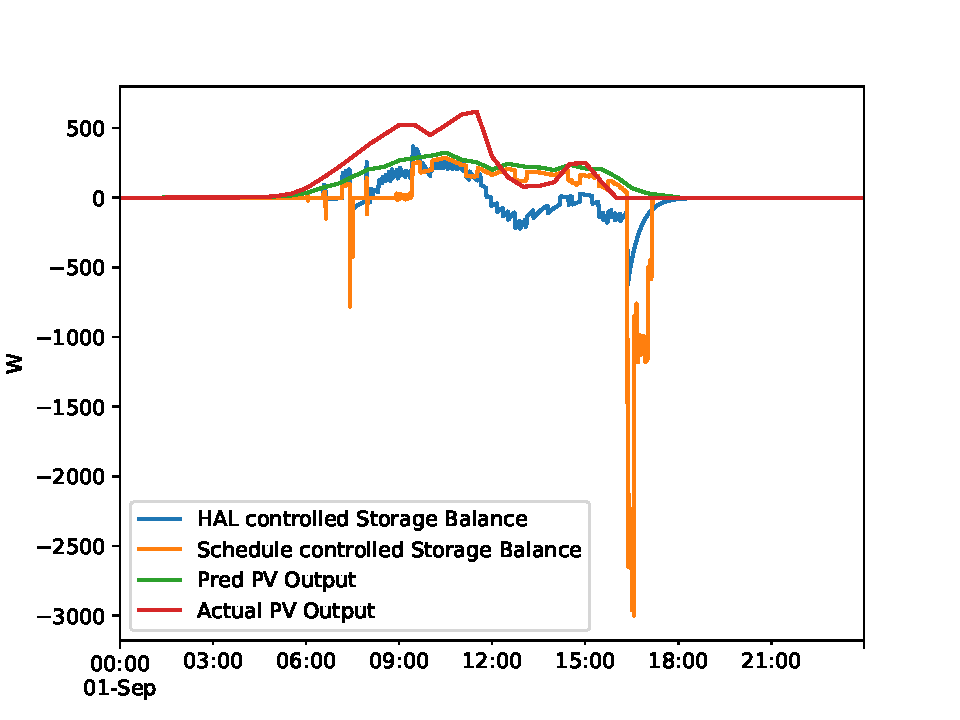
\includegraphics[width=\textwidth]{sept_real_example}
	\caption{Storage consumption and PV output during the first day of the September simulation. Around 9am, the HAL algorithm uses the peak in \ac{PV} production.}
	\label{f/res/real/example}
\end{figure}
\newpage
The simulation results of the second period (December) turned out to behave very similar to the simulations performed during September. However, in September the relative difference of the net import in the first (prediction data) and the second (real data) simulation run is $2.591\%$ whereas it is $0.046\%$ in December. Equation \ref{e/res/ratio} explains how these values were calculated with $n$ being the net import. This is likely due to the fact that there is a high thermal load and almost no \ac{PV} output. As a result, the \ac{PV} generated power is often instantly consumed by the heat pump which limits the algorithms ability to use the battery. A bigger \ac{PV} system or additional generators might create more interesting results.

\begin{equation}\label{e/res/ratio}
\frac{n^{Real OEMOF}}{n^{Real HAL}} - \frac{n^{Pred OEMOF}}{n^{Pred HAL}}
\end{equation}

\section{Schedule vs. Schedule Setup}
In the last setup HAL was not used as an online, near real time controller for the simulation with real \ac{PV} input data. Using the same method as before on the simulation results of \ac{OEMOF}, a schedule was created from HALs result on the predicted \ac{PV} data. As can be seen in figure \ref{f/res/svss/total}, this run results in slightly higher net import peak. However, Table \ref{t/res/schedule} shows that the total net import in the scheduled controlled run is less than in HALs online run on the prediction data while \ac{OEMOF}s schedule run has a higher total net import than in the prediction run. This could be an indicator that HAL created schedules can handle uncertainties better.
\begin{figure}[ht]
	\centering
	\subfloat[Total Net Import in .]{{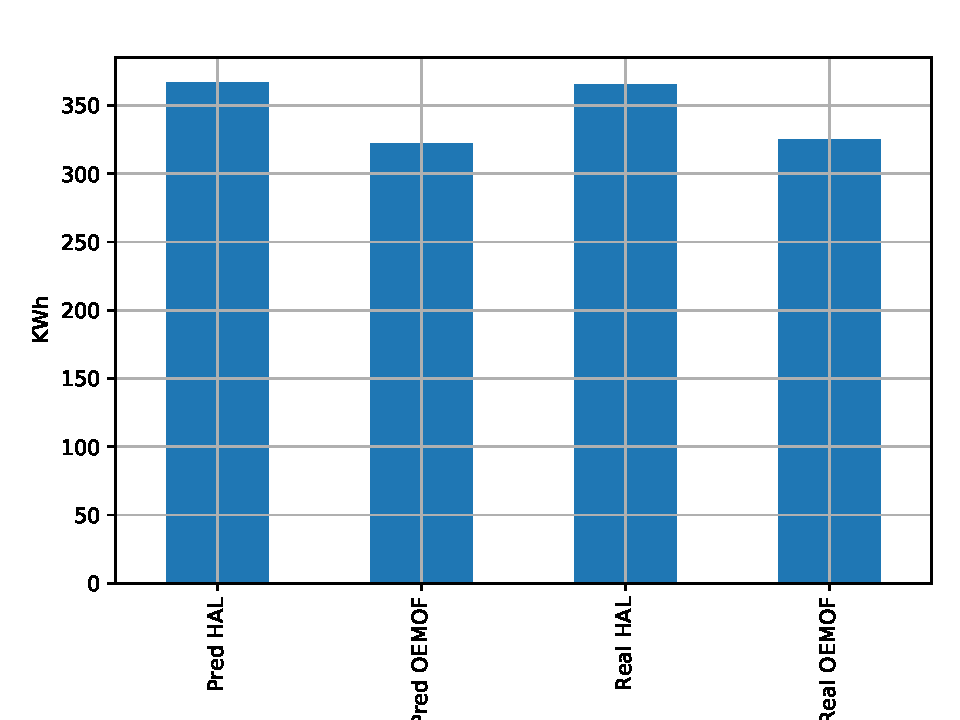
\includegraphics[width=0.465\textwidth]{sept_svss_total} }} % %\includesvg{image}
	%	\qquad
	\subfloat[Net Import Peak Distribution. Whiskers are 1.5 of the inter quantile range.]{{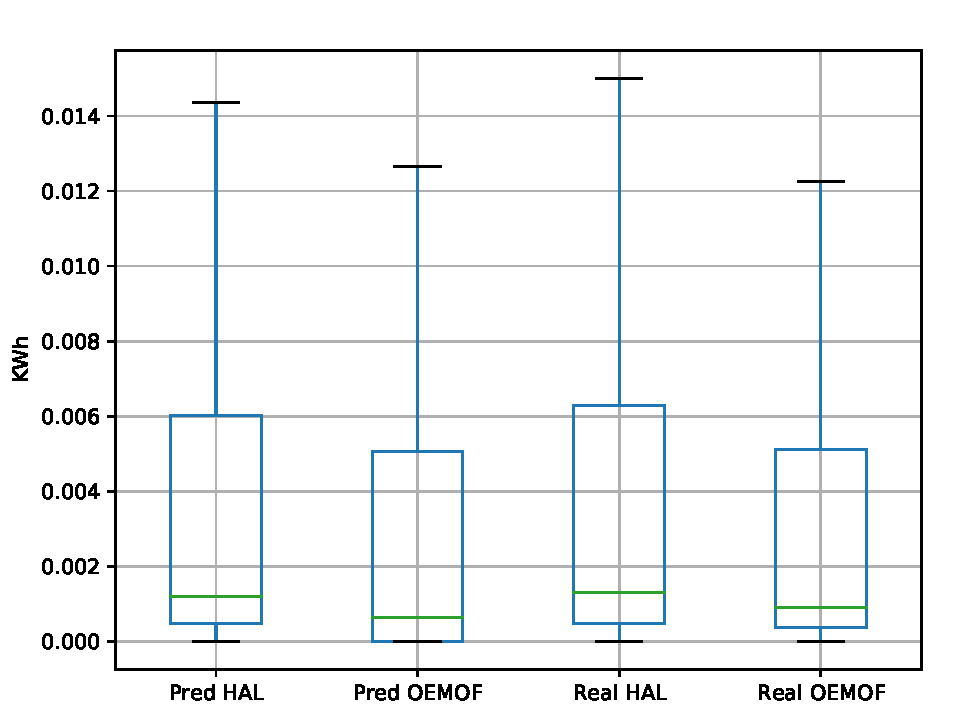
\includegraphics[width=0.465\textwidth]{sept_svss_peaks} }}%
	\caption{Simulation results with real PV and prediction data controlled by schedules. The second simulation runs (Real HAL, Real OEMOF) have a slightly higher total net import and more and higher peaks than the first simulation runs on the \ac{PV} prediction. }%
	\label{f/res/svss/total}%
\end{figure}

\begin{table}[h!]
\centering
\caption{Sum of all simulation runs net imports.}
\label{t/res/schedule}
\begin{tabular}{lr}
\toprule
{} &    sum \\
\midrule
Pred HAL   & 366.77 \\
Pred OEMOF & 322.48 \\
Real HAL   & 365.20 \\
Real OEMOF & 324.96 \\
\bottomrule
\end{tabular}
\end{table}


% --------------------------------------------------------------------------------------------
\chapter{Conclusions}\label{ch/conclusion}
% TODO
% We saw that splitting and uncertainty both reduce performance. However 12h split only by....
% reducing uncertainty in prediction by reducing optimization problem size and simulate a new prediction for the next optimization interval
This report should enable the reader to get an intuition about the properties of the two presented algorithms for controlling energy systems with sector coupling. 
These properties should be qualified to inform the reader about the application possibilities of a \ac{MILP} based optimization algorithm and an agent based supply and demand matching algorithm.
To compare complex energy systems, the HAL algorithm was extended to be able to model sector coupled devices.
A smart grid for a household was modeled, simulated and analyzed after performance metrics which were introduced.
Different test setups showed the properties of both algorithms with different scheduling horizons ranging from one month to one minute.

The incremental setup and the noise setup showed, that the performance of a schedule controlled energy system depends on the uncertainty of the input data.
By reducing the scheduling horizon to 6 hours, the uncertainty could be reduced with little impact on performance if the system resets during the night.
The greater the uncertainty in the predictions used for schedule creation, the better performs the HAL algorithm in comparison to long term schedules.
This is supported by the simulations performed with real \ac{PV} output data in the real data setup. This report only covers uncertainty in \ac{PV} data. In a real situation, the household demand is another major uncertainty factor in predictions.

The schedule vs. schedule setup showed that the HAL algorithm is not suitable to be used for long term scheduling horizons.

The noise setup shows how near realtime control strategies help to use unexpected short term changes in \ac{PV} output optimally. Although short term changes in pv power during the night won't happen in the real application, further research could show that clouds can likely cause similar effects during the day.
Another interesting research question is to find out how and if the optimal scheduling horizon correlates with the uncertainty in the input data used for schedule creation.

\bibliographystyle{plain}
\bibliography{references}

\clearpage

%%%%%%%%%%%%%%%%
%%% Abstract %%%
%%%%%%%%%%%%%%%%

\thispagestyle{empty}

\end{document}